\section{Results and Specific Discussion}
\subsection{\SI{}}

% TODO: Fit things to these power laws
\begin{figure}[t]
  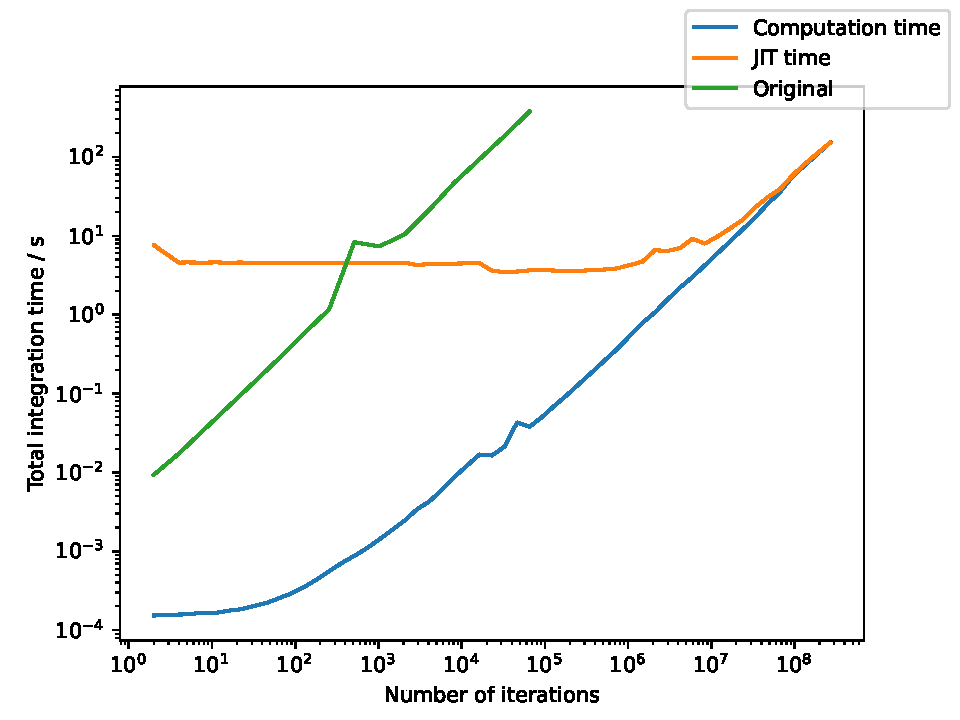
\includegraphics[width=\columnwidth]{figures/dho_n_runtime.pdf}
  \caption{A comparison of running a damped harmonic oscillator system for various numbers of iterations, with $r = 2, \Delta t = 0.1$ (Apple M1 Max, 64GB of ram). The \updimpl{} time is split into two components where \enquote{JIT time} represents the one time fixed cost of compiling the function and \enquote{Computation time} represents the actual time spent on computation.
  Each value is a mean of 4 runs, with the \orgimpl{} being cut off early due after $> 20$ minutes runtime for the the next sample. It can be seen, as expected, that the computation time for the \updimpl{} and the overall \orgimpl{} grow as a power law with $N$, while the JIT time remains roughly constant until growing as a power law from about $10^7$ iterations, where we estimate arrays become greater than 1Gb in size possibly hitting JAX de-optimisation.}
\end{figure}

\begin{figure}[t]
  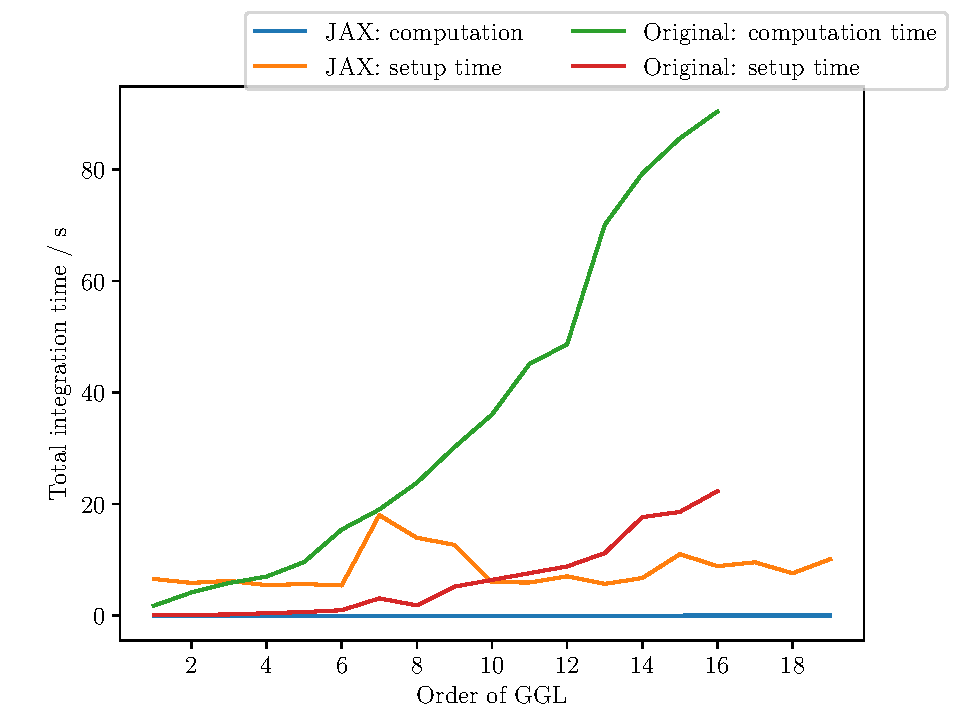
\includegraphics[width=\columnwidth]{figures/dho_r_runtime_linear.pdf}
  \caption{A comparison of running a damped harmonic oscillator system for various values of $r$, the order of the GGL quadrature, with $N_{\mathrm{iter}} = 500, \Delta t = 0.1$ (Apple M1 Max, 64GB of ram).
	For both implementations we split the overall time into setup and computation, each sampled 4 times, as changing the method order requires re-discretising the Lagrangian and thus non-trivial work under both implementations.}
% TODO: Talk about the bump around r=8
\end{figure}


\begin{enumerate}
	\item Error of method is preserved, energy error is bounded
	\item timestep count vs time for \orgimpl vs \updimpl
	\item r vs time for \orgimpl vs \updimpl
	\item Modelling of MD system
	\item PRD? for physics?
\end{enumerate}

% These are the error graphs similar to DTs paper (cite DT here)
% We got X% speed up
% This means we can model Y% larger systems for Z% longer time frames

\subsection{Loss Functions}

\begin{enumerate}
	\item Properties of the loss function
	\item Make a nice plot to show that they are well behaved around the true value (those ((2x2), 1) grids)
	\item 
\end{enumerate}

\subsection{PINN}

\begin{enumerate}
	\item Behaviour for different loss functions and emebeddings (agular!)
	\item Training loss things
	\item Preiction
\end{enumerate}

% This is the shit we got out of the method
% Essentially 
% Results of auto diff results with different loss functions
% If we can make those nice convergence/non-convergence Mandlebrot plots try that!

%\lipsum

\section{General Discussion}
% What do the pretty graphs actually mean in a broad sense
% Pull together with the background
% PHYSICS!!!

% Is this where we will mention the "future work" of NNs?

%\lipsum

\section{Conclusion}
